\documentclass[namedreferences]{solarphysics}

\usepackage[hyperref,optionalrh,showbiblabels]{spr-sola-addons} % For Solar Physics 
%\usepackage[optionalrh]{spr-sola-addons} % For Solar Physics 
%\usepackage{epsfig}          % For eps figures, old commands
\usepackage{graphicx}        % For eps figures, newer & more powerfull
%\usepackage{courier}         % Change the \texttt command to courier style
%\usepackage{amssymb}        % useful mathematical symbols
\usepackage{color}           % For color text: \color command
\usepackage{breakurl}        % For breaking URLs easily trough lines
\def\UrlFont{\sf}            % define the fonts for the URLs

\usepackage{graphicx}
\usepackage{pgfplots}
\usepackage{tikz}
\usepackage{gensymb}

\usepgfplotslibrary{dateplot}

\usepgfplotslibrary{external}
\usetikzlibrary{external}
\tikzsetexternalprefix{tikz/}
\tikzexternalize[shell escape=-enable-write18,optimize command away=\includepdf]

% General definitions
% please place your own definitions here and don't use \def but
% \newcommand{}{} or 
% \renewcommand{}{} if it is already defined in LaTeX

\newcommand{\BibTeX}{\textsc{Bib}\TeX}
\newcommand{\etal}{{\it et al.}}

% Definitions for equations
\renewcommand{\vec}[1]{{\mathbfit #1}}
\newcommand{\deriv}[2]{\frac{{\mathrm d} #1}{{\mathrm d} #2}}
\newcommand{\rmd}{ {\ \mathrm d} }
\newcommand{\uvec}[1]{ \hat{\mathbf #1} }
\newcommand{\pder}[2]{ \f{\partial #1}{\partial #2} }
\newcommand{\grad}{ {\bf \nabla } }
\newcommand{\curl}{ {\bf \nabla} \times}
\newcommand{\vol}{ {\mathcal V} }
\newcommand{\bndry}{ {\mathcal S} }
\newcommand{\dv}{~{\mathrm d}^3 x}
\newcommand{\da}{~{\mathrm d}^2 x}
\newcommand{\dl}{~{\mathrm d} l}
\newcommand{\dt}{~{\mathrm d}t}
\newcommand{\intv}{\int_{\vol}^{}}
\newcommand{\inta}{\int_{\bndry}^{}}
\newcommand{\avec}{ \vec A}
\newcommand{\ap}{ \vec A_p}

\newcommand{\bb}{\vec B}
\newcommand{\jj}{ \vec j}
\newcommand{\rr}{ \vec r}
\newcommand{\xx}{ \vec x}

% Definitions for the journal names
\newcommand{\adv}{    {\it Adv. Space Res.}} 
\newcommand{\annG}{   {\it Ann. Geophys.}} 
\newcommand{\aap}{    {\it Astron. Astrophys.}}
\newcommand{\aaps}{   {\it Astron. Astrophys. Suppl.}}
\newcommand{\aapr}{   {\it Astron. Astrophys. Rev.}}
\newcommand{\ag}{     {\it Ann. Geophys.}}
\newcommand{\aj}{     {\it Astron. J.}} 
\newcommand{\apj}{    {\it Astrophys. J.}}
\newcommand{\apjl}{   {\it Astrophys. J. Lett.}}
\newcommand{\apss}{   {\it Astrophys. Space Sci.}} 
\newcommand{\cjaa}{   {\it Chin. J. Astron. Astrophys.}} 
\newcommand{\gafd}{   {\it Geophys. Astrophys. Fluid Dyn.}}
\newcommand{\grl}{    {\it Geophys. Res. Lett.}}
\newcommand{\ijga}{   {\it Int. J. Geomagn. Aeron.}}
\newcommand{\jastp}{  {\it J. Atmos. Solar-Terr. Phys.}} 
\newcommand{\jgr}{    {\it J. Geophys. Res.}}
\newcommand{\mnras}{  {\it Mon. Not. Roy. Astron. Soc.}}
\newcommand{\nat}{    {\it Nature}}
\newcommand{\pasp}{   {\it Pub. Astron. Soc. Pac.}}
\newcommand{\pasj}{   {\it Pub. Astron. Soc. Japan}}
\newcommand{\pre}{    {\it Phys. Rev. E}}
\newcommand{\solphys}{{\it Solar Phys.}}
\newcommand{\sovast}{ {\it Soviet  Astron.}} 
\newcommand{\ssr}{    {\it Space Sci. Rev.}} 
\chardef\us=`\_

%%%%%%%%%%%%%%%%%%%%%%%%%%%%%%%%%%%%%%%%%%%%%%%%%%%%%%%%%%%%%%%%%%
\begin{document}

\begin{article}
\begin{opening}

\title{Characteristics of sunspots from the solar cycle 23}

\author[addressref=aff1]{\inits{A. E. S.}\fnm{A. E.}~\lnm{Spagiari}}%\sep
\author[addressref=aff2]{\inits{M. M.}\fnm{Mauricio}~\lnm{Marengoni}}%\sep
\author[addressref=aff3]{\inits{C. L. S.}\fnm{Caius}~\lnm{Selhorst}}%\sep
\author[addressref={aff1,aff2},corref,email={adrivalio@gmail.com}]{\inits{A. V.}\fnm{Adriana}~\lnm{Valio}}%\sep
%\author{\inits{}\fnm{}~\lnm{}\orcid{}}
%\author{P.~\surname{Author-a}$^{1}$\sep
%        E.~\surname{Author-b}$^{1}$\sep
%        M.~\surname{Author-c}$^{2}$      
%       }

%   \institute{$^{1}$ First affiliation
%                     email: \url{e.mail-a} email: \url{e.mail-b}\\ 
%              $^{2}$ Second affiliation
%                     email: \url{e.mail-c} \\
%             }
\address[id=aff1]{Centro de Rádio Astronomia e Astrofísica Mackenzie}
\address[id=aff2]{Escola de Engenharia Universidade Presbiteriana Mackenzie São Paulo Brazil}
\address[id=aff3]{Universidade Cruzeiro do Sul}

\runningauthor{Author-a et al.}
\runningtitle{Example paper}

\begin{abstract}
This work analyzed the physical characteristics of sunspots the solar cycle 23, detected using computer vision techniques.
Images in visible light and
magnetograms of the MDI instrument (Michelson Doppler Imager) of the space telescope
SOHO (Solar and Heliospheric Observatory) were used in the process of detecting
sunspots and the extraction of their characteristics. The flow of
solar irradiance, number of spots, number of sunspot groups, area, temperature, brightness and
the average magnetic field of sunspots were also studied. Based on the sunspot data, the behavior of these characteristics and relationships between them were verified along the
periods of solar minimum and maximum.

We detected and analyzed 32,317 sunspots, with longitude between -40\degree and 40\degree, throughout the entire solar cycle.
The daily Wolf number series was compared with data from the SIDC research center, and showed a 95\% correlation.
In addition, nonlinear correlations were found regarding area and extreme magnetic field, as well as regarding temperature and area, and finally regarding temperature and magnetic field.
It was also found that these correlations presented small variations over the time of the solar cycle 23, and that larger, colder sunspots and with stronger magnetic fields occur more frequently during periods of maximum activity.
\end{abstract}
\keywords{Sunspots, Cycle 23, Solar activity}
\end{opening}
%-------------------------------------------------

\section{Introduction}
     \label{S-Introduction} 
Sunspots are colder regions, therefore darker, found on the photosphere of the Sun.
This phenomenon is associated with changes in the solar magnetic field and its activity cycle.
Galileo Galilei, among others, observed sunspots through telescopes around 1610 \citep{Eddy1976}.
Since then, sunspots have been studied in detail in relation to their quantity in the solar disk and their area \citep{Hathaway2015}.

Continuous observation of sunspots since the 17th century has shown a cyclic behavior of solar activity,
ranging between periods with few sunspots and others with many sunspots at intervals of approximately eleven years \citep{Hathaway2015}.
During high solar activity periods, phenomena such as solar flares and coronal mass ejections are frequent and their effects cause a range of disturbances in our planet.

Sunspots evolve and dissipate in active regions.
Generally, more than one spot share the same active region.
This conglomerate of spots connected to the same active region is called a group of spots.
Because they are part of the same active region and are subjected to the same configuration of magnetic field arrangements,
these spots share similar physical characteristics such as lifetime and spatial location \citep{curto2008}.

Sunspots characteristics and their relations have been studied over the years.
In \citeyear{Dicke1970}, \citeauthor{Dicke1970} described the temperature of a sunspot as a function of the square of its magnetic field.
In recent years, several studies have been carried out to investigate the characteristics and behavior of sunspot.
In \citeyear{Kopp1992}, \citeauthor{Kopp1992} investigated the relationship between magnetic field strength and temperature in the sunspot region and they found a nonlinear relationship between magnetic field strength and the sunspot brightness.
These results are in agreement with results obtained by \citealp{Dicke1970}.
\citealp{Penn2006} analyzed about 900 sunspots between 1998 and 2005,
observing changes in the magnetic field and the sunspots temperature,
and the results found were similar to \citealp{Kopp1992}.

\citealp{Javaraiah2013} investigated the variation of the sunspot area.
Groups of sunspots data were analyzed from 1874 to 2011,
which led to the discovery of a more comprehensive variation in solar activity, 
with a possible cycle of approximately forty-four years.
Additionally, they may reveal clues to the functioning of the solar dynamo. 
In the same year, \citealp{Toma2013}, published the results of their study about the evolution of sunspot areas on solar cycles 22 and 23,
concluding that there was a significant decrease in the sunspot area of cycle 23 compared to cycle 22.
The authors argued that this decrease might be indicative of changes in the solar dynamo.

Techniques of computational vision for segmentation and automatic extraction of sunspots,
as well as analysis of its characteristics,
have been applied in the last years with high levels of correlation to official indexes.
In \citeyear{zharkova2003}, \citeauthor{zharkova2003} used the Canny edge detection algorithm to discover the spots contours.
\citealp{zharkov2005}, presented a technique of detection of sunspots using the Sobbel algorithm,
morphological filters, binarization and an image pre-processing for removal of noise and attenuation of the effect of limb darkening.
\citealp{colak2007}, argued about the use of data obtained through the use of computational techniques for the prediction of space weather.
In the following year \citealp{curto2008}, presented an algorithm based on techniques of binarization and mathematical morphology,
these ideias were implemented in more recent works, for example by \citealp{spagiari2012} and \citealp{curto2008}.

This work uses mathematical morphology,
a computer vision technique, 
for spot detection and automatic extraction of sunspot characteristics in solar disk images.
To extract the relevant characteristics of the detected solar spots, such as area, temperature, 
contrast and intensity of the magnetic field, we used images of the MDI (Michelson Doppler Imager)
instrument found in the SOHO satellite (Solar and Heliospheric Observatory)
using white light and the magnetogram produced.
The research was performed for the entire solar cycle 23 and analyzes the temporal evolution of physical
parameters of the spots and additionally compare whether there are alterations in the known correlations 
between these characteristics during the course of the solar cycle.

\section{Observations}
\label{S-obs}
In 1995, NASA launched the SOHO (Solar and Heliospheric Observatory) satellite to observe the Sun using different instruments, including the MDI (Michelson Doppler Imager),
a 1024x1024 pixel CCD camera that observes the Sun at visible wavelengths and detects sunspots without the interference of the terrestrial atmosphere, with high spatial performance \citep{scherrer1991}.

This work uses as input data images of the MDI (Michelson Doppler Imager) instrument from the SOHO space satellite.
The MDI obtains as main products the image of the solar disk in white light and the magnetogram, a spatial representation of the intensity of the solar magnetic field \citep{scherrer1991}.
An example of these images is seen in Figure~\ref{fig1}.

To extract the desired information for a given day, 
it is necessary to use a pair of images from the visible light and the magnetogram.
These images should be separated by the shortest possible time since the two observations do not occur at the same instant.
On SOHO images database, these two observations are generally thirty seconds apart.
  
  \begin{figure}
                                % includes the two top panels 
   \centerline{\hspace*{0.015\textwidth}
               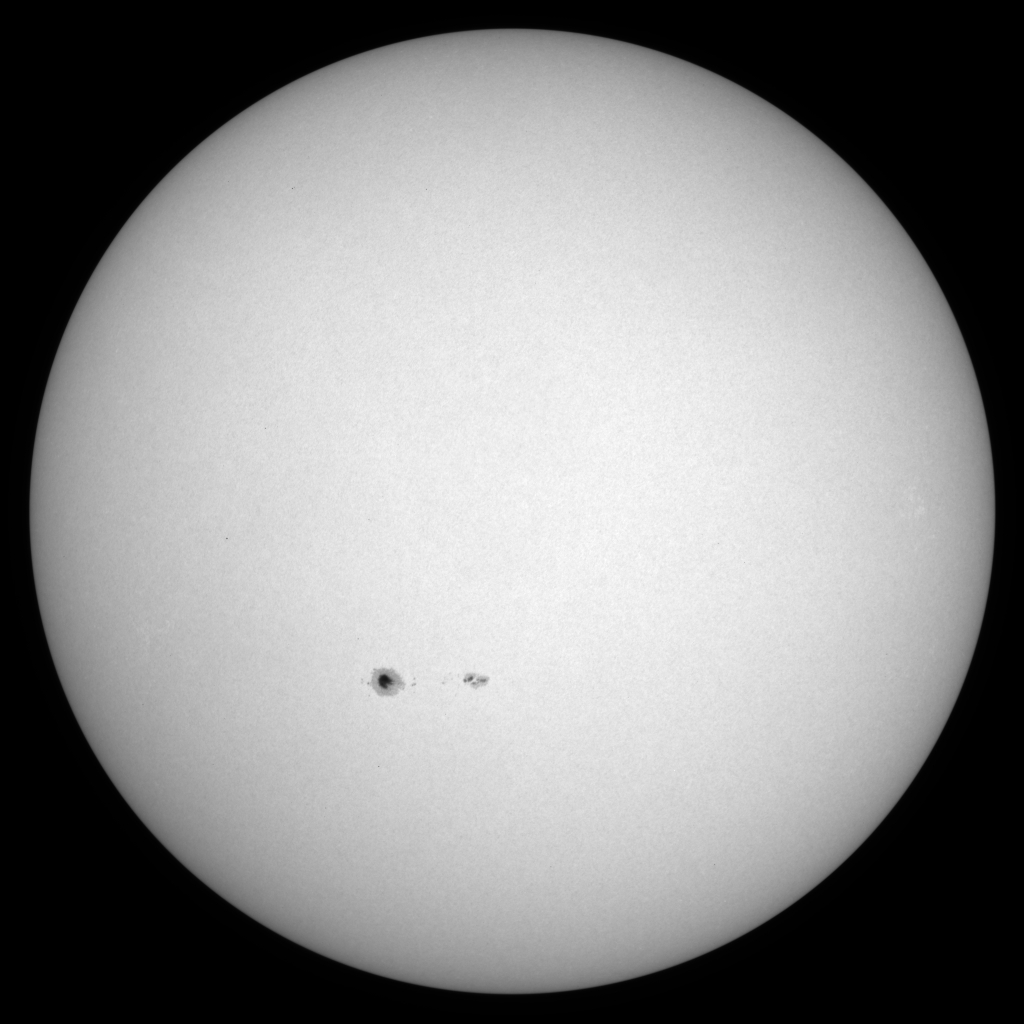
\includegraphics[width=0.515\textwidth,clip=]{./img/20060816.jpg}
               \hspace*{-0.03\textwidth}
               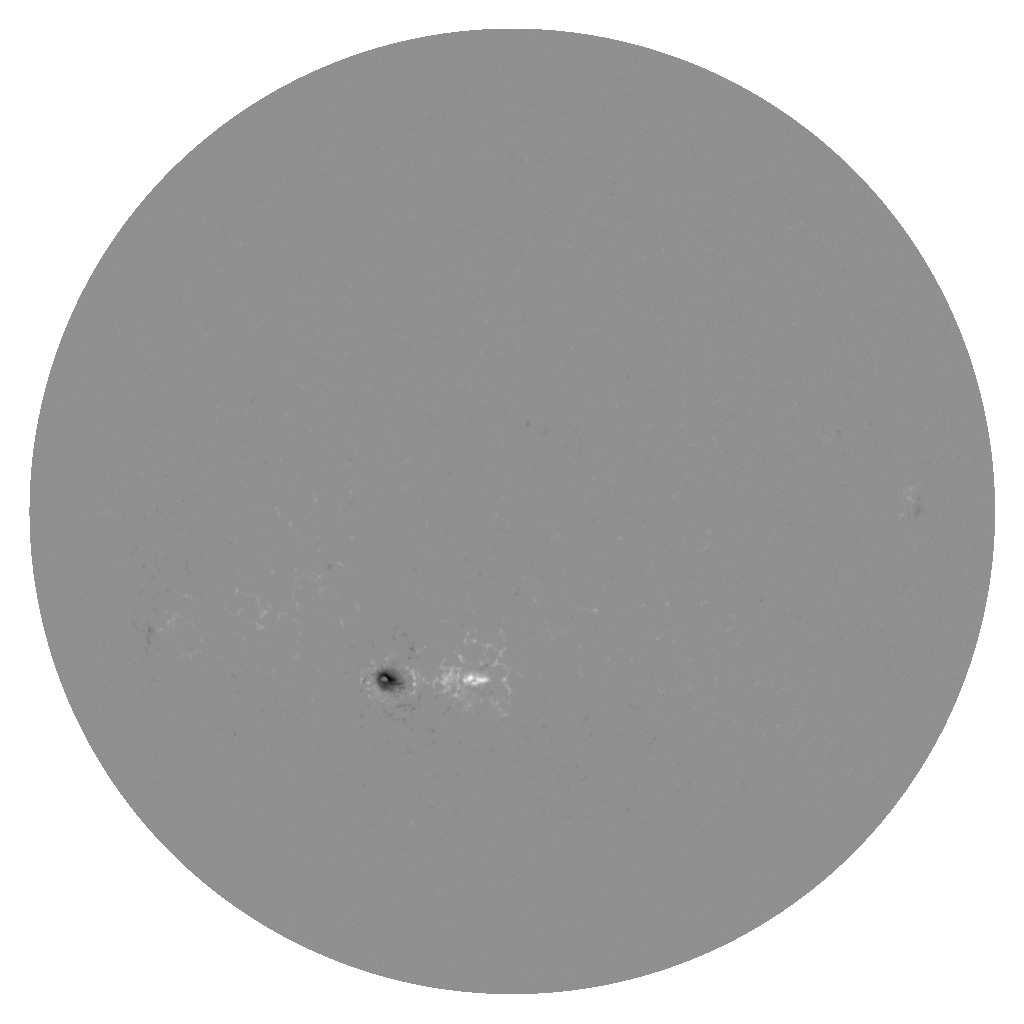
\includegraphics[width=0.515\textwidth,clip=]{./img/20060816_mag.jpg}
              }
     \vspace{-0.50\textwidth}   % Shift close to the panel top 
     \centerline{\Large \bf     % Includes the labels (here needs the color 
                                %   package, see beginning of this file)
      \hspace{0.0 \textwidth}  \color{white}{(a)}
      \hspace{0.415\textwidth}  \color{black}{(b)}
         \hfill}
     \vspace{0.46\textwidth}    % Shift back to the panel bottom 
              
\caption{Sun image in visible light from SOHO (a) and the magnetogram (b), both obtained by the MDI in 08/26/2006.
        }
   \label{fig1}
   \end{figure}

\section{Methodology} %%%%%%%%%%%%%%%%%%%%%%%%%%%%%%%%%%%%%%%%
      \label{S-meth}      

\subsection{Automatic solar sunspot detection} %%%%%%%%%%%%%%
  \label{S-detect}
In the last years, some techniques of computer vision have been applied to the problem of automatic detection of sunspots, obtaining satisfactory results.
\citealp{zharkov2005}, used image-processing techniques to remove noise and details of no interest and,
after preprocessing, they used Sobel's edge detection algorithm to determine candidate spots as potential sunspots.
Another approach by \citealp{curto2008},
using images from the Ebro observatory, proposed a technique employing mathematical morphology as an attempt to detect the entire pattern of a perimeter, sometimes amorphous, of sunspots.

For the detection of sunspots, an algorithm based on binarization and mathematic morphology was used,
based on the method used by \citealp{curto2008},
and adapted for the images of the SOHO observatory.
The sunspot detection algorithm receives as a parameter an image of the complete solar disk in JPG format and returns a binary processed image of the same size as the original.
The pixels detected as belonging to a sunspot are white,
and the detected pixels not belonging to any sunspot are black.

The main steps for detecting sunspots are the bottom-hat transform, the binarization and the morphological aperture \citep{spagiari2012}.
Some parameters are necessary to accomplish these operations.
The morphological operations require the format and size of the structuring element (BSS).
The shape of the structuring element used was elliptical,
and the ideal size of the structuring element was found by an algorithm, 
starting with a minimum size of 3x3 pixels.
The ideal cut-off parameter for binarization (BT) is also estimated by the sunspot detection algorithm.

\subsection{Physical characteristics of solar spots} %%%%%%%%%%%%%%
  \label{S-phy}
The indicators for spots were extracted using monthly images from SOHO throughout solar cycle 23,
from May 1996 to April 2008.
The white light image from MDI/SOHO is converted to JPG format to use in computer vision processes and its original FITS format is used to extract the physical characteristics of sunspots, 
since the FITS format maintains important information about observation time as well as the absolute value of pixel intensity, different from the JPG format, which stores only the relative pixel intensity.
The magnetogram is also used as complementary data, from which magnetic field intensities are extracted from spot regions.
The parameters of the sunspots extracted from the images were location, area, relative intensity, temperature, magnetic field, and central intensity of the disk at the time of observation.
The characteristics of each set of images were extracted and stored as a time series.

The area of the sunspot is estimated by the sunspot detection algorithm.
The sunspot area in $m^2$ is calculated by Equation~\ref{eq:area}.
The parameter $p$ is sunspot number of pixels,
whereas $\theta$ is the angular size of the pixels in arcseconds from the FITS file header,
$d$ is the distance from SOHO satellites to the sun and $l$ and $b$ are,
respectively, the latitude and longitude of the sunspot in heliographic coordinates.

\begin{equation} \label{eq:area}
\label{eq:area}
    \mathit{s = p\left (\frac{\frac{\theta}{3600}\frac{\pi}{180}d}{\cos(l)\cos(b)} \right)}^{2} m^2
\end{equation}

The intensity of the sunspot is obtained through the average of the intensities of the spot pixels read from the image file of the solar disk in white light and in FITS format.
This definition is formalized in Equation~\ref{eq:int},
where $I_{p}$ is the intensity set of the $p$ pixels that make up the sunspot and $I_{c}$ is the mean intensity of the center of the solar disk.
The intensity of the center of the Sun, $I_{c}$, is obtained by means of the white light image of the solar disk in the FITS format.
A simple average of the pixels belonging to an area of approximately $10^5 m^2$,
originating in the center of the solar disk is calculated.
The average of a small portion of pixels in the central region of the Sun provides a reliable estimate of the intensity of the Sun’s center.
Images with sunspots in that region have been discarded.

\begin{equation} \label{eq:int}
    \mathit{f_{i} = \frac{1}{I_{c}} \left (  \sum_{0}^{p} I_{p} \right )\frac{1}{p}}
\end{equation}

The temperature of all detected sunspots is calculated by substituting the mean intensity (Equation~\ref{eq:int}) in Equation~\ref{eq:temp}.

\begin{equation} \label{eq:temp}
    \mathit{T_{m} = \frac{h\upsilon}{K_{b}} \left [\ln\left ( 1 + \frac{e^{\frac{h\upsilon}{K_{b}T_{c}}} - 1}{f_{i}} \right ) \right ]^{-1}}
\end{equation}

For the analysis of the magnetic field of a certain sunspot, three values are obtained: the average magnetic field,
the maximum magnetic field, and the minimum magnetic field.
The magnetic field of the sunspot is estimated among the position data of the pixels belonging to the sunspot and obtained by the algorithm of detection of sunspots.
The algorithm is used with the solar disk magnetogram in FITS format. 
It is important that the magnetogram and the white light image analyzed are separated by the shortest possible time to minimize the effects of solar rotation.
This work used only sets of images with intervals of observation less than thirty minutes.

For the magnetogram in the FITS format, the value corresponding to each pixel represents the intensity of the magnetic field in the region.
For each pixel of the set of pixels that make up a sunspot,
it is analyzed the value corresponding to that pixel in the magnetogram,
and thus a mean of all pixels read is obtained, that is, the pixel with the highest intensity and the one with the least intensity.

In the magnetogram, the intensity value of the magnetic field is always in reference to the observer and we need to correct this value of intensity by the projection effects for the coordinate of the sunspot.
For this correction was used Equation~\ref{eq:b}, where $\theta$ is the heliographic angle of the sunspot and $B_z$ is the intensity of the magnetic field obtained in the magnetogram \citep{borrero2011}.

\begin{equation} \label{eq:b}
    \mathit{B = \frac{B_z}{\cos\theta}}
\end{equation}

The magnetogram produced by the MDI instrument from SOHO may shows saturation in regions where the magnetic field strength exceeds 2000 Gauss,
so the data of extreme magnetic field with intensity above 2000 Gauss can be underestimated \citep{selhorst2008}.
    
\section{Results} %%%%%%%%%%%%%%%%%%%%%%%%%%%%%%%%%%%%%%%%
      \label{S-results}      

\subsection{Cycle 23} %%%%%%%%%%%%%%
  \label{S-cycle23}
This work processed 6,870 images of the SOHO observatory, which represent a daily sample of images of the Sun for the period corresponding to the solar cycle 23.
A total of 32,317 sunspots with a longitude between -40\degree and 40\degree were detected and analyzed.
A plot of the number of the Wolf number obtained from these spots is shown in Figure~\ref{gr:ciclo23}, where the 11 year sola activity cycle is clearely seen.

\begin{figure} [!htbp]
\begin{tikzpicture}
\begin{axis}[
        width=350pt,
        height=216pt,
        no markers,
        date coordinates in=x,
        xticklabel=\month-\year,
        xmin={1996-08-01},
        xmax={2008-01-31},
        xticklabel style= {rotate=45,anchor=north east},
        ylabel= Wolf number]
    \addplot table [x=Data, y=MACK5] {data/ciclo23.txt};
    %\addlegendentry{MACK5}
    %\addplot table [x=Data, y=SIDC] {data/ciclo23.txt};
    %\addlegendentry{SIDC}
\end{axis}
\end{tikzpicture}
\caption{Daily comparison of sunspot detection results for the solar cycle 23}
\label{gr:ciclo23}
\end{figure}

The temporal evolution of the physical parameters of the spots such as area, contrast and extreme magnetic field are shown in Figures~\ref{fig:c23a},~\ref{fig:c23c} and~\ref{fig:c23b}, respectively.
Note that these physical characteristics volve during the solar cycle, as can be seen from Figures~\ref{fig:c23a} -~\ref{fig:c23b}.
During the period of maximum activity, from 1999 through 2004, the larger, cooler solar sunspots with intense magnetic fields occurred with higher frequency.
A small variation in the mean value of the contrast is noted, the spots being darker at the maximum of the solar cycle 23.
Moreover, the average value of the sunspot temperature is $100 K$ colder during the maximum of the solar cycle 23.

\begin{figure}[!htbp]
\begin{tikzpicture}
\input ciclo23_area.tex
\end{tikzpicture}
\caption{Daily evolution of the sunspot area along the solar cycle 23.}
\label{fig:c23a}
\end{figure}

\begin{figure}[!htbp]
\begin{tikzpicture}
\input ciclo23_contrates.tex
\end{tikzpicture}
\caption{Daily evolution of the sunspot contrast along the solar cycle 23.}
\label{fig:c23c}
\end{figure}

\begin{figure}[!htbp]
\begin{tikzpicture}
\input ciclo23_bmax.tex
\end{tikzpicture}
\caption{Daily evolution of the sunspot Extreme magnetic field along the solar cycle 23.}
\label{fig:c23b}
\end{figure}

\subsection{Histogram} %%%%%%%%%%%%%%
  \label{S-hist}
The following physical parameters were extracted from the detected sunspots: area, contrast, temperature and extreme magnetic field. 
Each of the extracted features was independently analyzed, and their mean values obtained from the statistical distribution of each parameter using histograms.

Figure~\ref{fig:h}a shows the histogram of the spots log area for the solar cycle 23.
As can be seen, the areas of the sunspots vary by a factor of 100, the smaller spots being much more abundant.
During the period of minimum activity (2005-2008), there appears to be a second component of spots larger than $10^8 m^2$ (Figure~\ref{fig:h}b)

  \begin{figure}[!htbp] 
                                % includes the two top panels 
   \centerline{\hspace*{0.015\textwidth}
               \begin{tikzpicture}
                   \input hist_area.tex
               \end{tikzpicture}
               \hspace*{-0.03\textwidth}
               \begin{tikzpicture}
                   \input hist_area_p4.tex
               \end{tikzpicture}
              }
     \vspace{-0.40\textwidth}   % Shift close to the panel top 
     \centerline{\Large \bf     % Includes the labels (here needs the color 
                                %   package, see beginning of this file)
      \hspace{0.0\textwidth}  \color{black}{(a)}
      \hspace{0.390\textwidth}  \color{black}{(b)}
         \hfill}
     \vspace{0.36\textwidth}    % Shift back to the panel bottom 
              
\caption{Histogram of the area of the sunspots. (a) cycle 23, (b) 2005-2008.}
   \label{fig:h}
   \end{figure}

Figure~\ref{fig:cont} shows the contrast histogram for the spots of the solar cycle 23. 
The contrast of the sunspots for the solar cycle 23 shows a mean value of 0.78 + 0.11.

\begin{figure}[!htbp] 
    \centerline{
        \begin{tikzpicture}
            \input hist_contraste.tex
        \end{tikzpicture}}
    \caption{Contrast histogram of spots for the entire solar cycle 23}
    \label{fig:cont}
\end{figure}

Figure~\ref{fig:temp} shows the histogram of the spot temperature for the solar cycle 23 calculated from its intensity, using Equation~\ref{eq:temp}.
The temperature has the mean value of $5400 \pm 200K$.
As seen in the contrast histogram, the spot temperature distribution has a second, colder component. The origin of this component is unknown.

\begin{figure}[!htbp] 
    \centerline{
        \begin{tikzpicture}
            \input hist_temp.tex
        \end{tikzpicture}}
    \caption{histogram of the spot temperature for the entire solar cycle 23}
    \label{fig:temp}
\end{figure}

Figure~\ref{fig:mag} shows the histogram of the maximum magnetic field of the sunspots for the solar cycle 23.
This parameter presents a mean value of $1700 \pm 600G$ for the maximum magnetic intensity of sunspots.

\begin{figure}[!htbp] 
    \centerline{
        \begin{tikzpicture}
            \input hist_mag.tex
        \end{tikzpicture}}
    \caption{Histogram of the maximum magnetic field of the sunspots for the entire solar cycle 23}
    \label{fig:mag}
\end{figure}

\subsection{Correlations} %%%%%%%%%%%%%%
The correlation analysis between the characteristics of the spots was performed using the monthly sample of sunspots.
We used 2,132 spots detected on days 1 and 15 of each month that compose the solar cycle 23.

The dispersion graph of Figure~\ref{fig:txa} between temperature and area (on a log scale) shows that the temperature of the sunspot has a relation to its area,
where larger sunspots are consistently colder than smaller sunspots.
The same correlation can be verified in the scatter plot of Figure~\ref{fig:cxa} between area and contrast. 
This occurs because the temperature is calculated from the intensity (Equation~\ref{eq:temp}).
Again, the presence of a second component of colder ($T <5300K$) and darker spots (contrast $<0.7$) is noted.

\begin{figure}[!htbp] 
    \centerline{
        \begin{tikzpicture}
            \input tempxarea.tex
        \end{tikzpicture}}
    \caption{Dispersion graph of sunspot temperature by sunspot area for solar cycle 23}
    \label{fig:txa}
\end{figure}

\begin{figure}[!htbp] 
    \centerline{
        \begin{tikzpicture}
            \input contxarea.tex
        \end{tikzpicture}}
    \caption{Dispersion graph of sunspot contrast by sunspot area for solar cycle 23}
    \label{fig:cxa}
\end{figure}

The dispersion graph of Figure 32 between extreme magnetic field and temperature matches the results of \citealp{Dicke1970}, and \citealp{Kopp1992}, 
showing a nonlinear relationship between magnetic field and temperature.
The red adjusted line is based on Equation~\ref{eq:dicke} \citep{Dicke1970}:
\begin{equation} \label{eq:dicke}
    \mathit{\frac{T}{Te}= -3.21\times 10^{-8}B^{2} + 0.95}
\end{equation}

A generalized form of Equation~\ref{eq:dicke},
$T / T_e = aB^2 + c$, was fitted to the data extracted by this work,
resulting in values of a = $-1.08 \times 10^{-8}$ and $c = 0.98$ (green line). 
Note that the sunspots adjusted by \citealp{Dicke1970}, were cooler and presented less intense magnetic fields than those detected in the solar cycle 23.

\begin{figure}[!htbp] 
    \centerline{
        \begin{tikzpicture}
            \input tempxbmax.tex
        \end{tikzpicture}}
    \caption{Dispersion graph of sunspot temperature by sunspot extreme magnetic field for solar cycle 23}
    \label{fig:cxa}
\end{figure}

The scattering graph between area and extreme magnetic field can be observed in Figure~\ref{fig:axb}.
By analyzing separately the positive and negative components of the extreme magnetic field of each sunspot,
it is observed that both components are related to the area, shown through an adjusted curve in orange.

\begin{figure}[!htbp] 
    \centerline{
        \begin{tikzpicture}
            \input areaxbmax.tex
        \end{tikzpicture}}
    \caption{Dispersion graph of sunspot area by sunspot extreme magnetic field for solar cycle 23}
    \label{fig:axb}
\end{figure}

\section{Conclusion} %%%%%%%%%%%%%%%%%%%%%%%%%%%%%%%%%%%%%%%%
      \label{S-Conclusion} 
The objective of this work was to automatically detect and extract characteristics of sunspots along the whole solar cycle 23,
obtained from SOHO satellite images. The study of these characteristics behavior is important to understand other phenomena related to the solar activity and the solar dynamo.
We also analyzed the existence of correlations between the physical properties of the spots.

Mathematical morphology was used for the detection of sunspots,
a versatile computational vision technique used both for noise filtering and for enhancement of areas of interest obtained from images.
The algorithm used in this work was inspired by the algorithm developed by \citealp{curto2008}.
A program was developed that implements the algorithms and the methodology is described in this work. 
A total of 6,870 images of the complete solar disk were processed from July 1997 to January 2008, 
which comprises the solar cycle 23,
and detected 32,317 solar spots, with a longitude between -40\degree and 40\degree.

Based on the physical characteristics extracted from the detected sunspots,
a quadratic correlation was verified between the temperature and the sunspots magnetic field. 
This correlation was also found by \citealp{Kopp1992}, 
and earlier \citealp{Dicke1970} described this nonlinear correlation with the sunspot temperature as a function of the square of its magnetic field,
as can be seen in Equation 16. The adjustment using equation $aB^2 + c $ to the data extracted by this work resulted in parameters a and c close to those calculated by \citealp{Dicke1970}.
Linear correlations were also found between the logarithm of the area and the extreme magnetic field, 
as well as between temperature and the log of the area.

As for the temporal evolution of the physical parameters of sunspots, we noted that during periods of maximum activity,
the spots are larger, colder and showed more intense magnetic field than at the beginning or at the end of solar cycle 23.

%%%%%%%%%%%%%%%%%%%%%%%%%%%%%%%%%%%%%%%%%%%%%%%%%%%%%%%%%%%%%%%%%%%%%%%%%%%
\begin{acks}
 The authors thank ... ({\it note the reduced point size})
\end{acks}

\noindent To change a title use an optional parameter:\par
\verb+\begin{acks}[Acknowledgements]...\end{acks}+



%\acknowledgment US spelling: \verb+\acknowledgment+
%\acknowledgement British  spelling: \verb+\acknowledgement+

%%%%%%%%%%%%%%%%%%%%%%%%%%%%%%%%%%%%%%%%%%%%%%%%%%%%%%%%%%%%%%%%%%%%%%%%%%%
     % format of references provided by the journal (.bst)
\bibliographystyle{spr-mp-sola}
     % name your Bibtex file containing your references (.bib)
\bibliography{biblproj}  

     % Checking: look if the file containing the ``\bibitem'' exits
     %           so check if the .bbl file exist (bibTeX compilation)
\IfFileExists{\jobname.bbl}{} {\typeout{}
\typeout{****************************************************}
\typeout{****************************************************}
\typeout{** Please run "bibtex \jobname" to obtain} \typeout{**
the bibliography and then re-run LaTeX} \typeout{** twice to fix
the references !}
\typeout{****************************************************}
\typeout{****************************************************}
\typeout{}}

\end{article} 

\end{document}
